\documentclass[10pt,letterpaper]{article}
\usepackage{url}
\usepackage{cogsci}
\usepackage{graphicx}
\usepackage{pslatex}
\usepackage{apacite2}
\usepackage{float}
\usepackage{amssymb}
\usepackage{amsmath}
\usepackage{natbib}
\usepackage[usenames,dvipsnames]{color}
\usepackage{stfloats}
\usepackage{booktabs}
\usepackage{multirow}

\title{The Divergent Lexicon: Lexical Overlap Decreases With Age in a Large Corpus of Conversational Speech}
 
\author{{\large \bf Stephan C. Meylan (smeylan@berkeley.edu)} \\
Department of Psychology, University of California, Berkeley, CA 94720 USA\\
\\
{\large \bf Susanne Gahl (gahl@berkeley.edu)} \\
Department of Linguistics, University of California, Berkeley, CA 94720 USA \\
}


\begin{document}
\renewcommand{\baselinestretch}{0.97}

\maketitle

\begin{abstract}
Changes in language processing and production accompanying aging have most commonly been interpreted as evidence for age-related cognitive decline. A recent proposal \citep{ramscarEtAl2014} challenges that interpretation, asserting instead that such changes emerge as a consequence of---and in order to support---processes of lifelong learning like continued vocabulary growth. Under this account, the mechanisms of language processing and production do not deteriorate with age, but rather the computational complexity of the underlying information processing task increases as more data is observed over the lifespan. The current study examines whether spoken language displays properties consistent with the notion of lifelong learning by examining the relationship between age, within-speaker lexical diversity, and between-speaker lexical overlap in a conversational speech corpus, Switchboard I. We find older speakers exhibit more diverse lexicons, and that they share fewer words with interlocutors than younger speakers. 
%

\textbf{Keywords:} 
lexicon; aging; corpus linguistics; speech
\end{abstract}

\begin{table*}[b]
\centering
\begin{tabular}{ l | c | c | c | c | r }
    & Speaker 1  & Speaker 2 & Lex. Div 1 & Lex. Div 2 & Jaccard Index\\
    \hline
  Case 1 & \colorbox{red}{\textcolor{white}{AA}} \colorbox{blue}{\textcolor{white}{BBB}} \colorbox{green}{\textcolor{white}{CC}} \colorbox{BurntOrange}{\textcolor{white}{D}} \colorbox{cyan}{\textcolor{white}{E}} & \colorbox{red}{\textcolor{white}{A}}  \colorbox{blue}{\textcolor{white}{BBB}} \colorbox{green}{\textcolor{white}{CC}} \colorbox{OliveGreen}{\textcolor{white}{FF}} \colorbox{OrangeRed}{\textcolor{white}{G}} & .56 ($5/9$) & .56 ($5/9$) & .43 ($3/7$)  \\
  Case 2 & \colorbox{red}{\textcolor{white}{AA}} \colorbox{blue}{\textcolor{white}{BB}} \colorbox{green}{\textcolor{white}{C}} \colorbox{BurntOrange}{\textcolor{white}{D}} \colorbox{cyan}{\textcolor{white}{E}} \colorbox{DarkOrchid} {\textcolor{white}{H}} \colorbox{Emerald}{\textcolor{white}{I}} & \colorbox{red}{\textcolor{white}{A}}  \colorbox{blue}{\textcolor{white}{BB}} \colorbox{green}{\textcolor{white}{C}} \colorbox{OliveGreen}{\textcolor{white}{FF}} \colorbox{OrangeRed}{\textcolor{white}{G}} \colorbox{RoyalPurple}{\textcolor{white}{J}} \colorbox{Dandelion}{\textcolor{white}{K}}  & .78($7/9$) & .78 ($7/9$) & .27 ($3/11$)  \\
  Case 3 & \colorbox{red}{\textcolor{white}{AA}} \colorbox{blue}{\textcolor{white}{BB}}  \colorbox{green}{\textcolor{white}{C}}  \colorbox{BurntOrange}{\textcolor{white}{D}} \colorbox{cyan}{\textcolor{white}{E}} \colorbox{DarkOrchid} {\textcolor{white}{H}} \colorbox{RoyalPurple}{\textcolor{white}{J}} &  \colorbox{red}{\textcolor{white}{A}} \colorbox{blue}{\textcolor{white}{BB}} \colorbox{green}{\textcolor{white}{C}} \colorbox{OliveGreen}{\textcolor{white}{FF}}  \colorbox{cyan}{\textcolor{white}{E}} \colorbox{DarkOrchid} {\textcolor{white}{H}} \colorbox{Dandelion}{\textcolor{white}{K}} & .78 ($7/9$) & .78 ($7/9$) & .55 ($5/9$)  \\	  
  \\
\end{tabular}
\caption{This toy example demonstrates how an increase in lexical diversity (Uber Index) may co-occur with either a decrease in lexical overlap between speakers (Case 1$\rightarrow$ Case 2) or an increase in lexical overlap (Case 1 $\rightarrow$ Case 3). Individual letters represent tokens; types are grouped by color. The Jaccard index, a measure of similarity between speakers, is calculated as the number of types in the intersection between speakers divided by the number of types in the union. }
\label{tab:diversityAndOverlap}
\end{table*}


\section{Introduction}
%GENERAL SLOWDOWN
Age heralds, at least on first glance, a decline in speakers' language abilities: older adults are slower to recognize words \citep{spielerBalota2000}, experience more tip-of-the-tongue states in which they cannot produce the correct word \citep{brownNix1996}, have a higher rate of disfluencies in conversational speech than their younger counterparts \citep{hortonEtAl2010}, and perceive a decline in their own language abilities \citep{ryanEtAl1992}. Many of these declines implicate changes in processing and production related specifically to words, necessitating a theory of how lexical processing and production may change as speakers age.

Established theories that account for slowing in lexical processing, as described in \citet{thorntonLight2006}, include the \textit{inhibition deficit hypothesis}, that  older adults are less able to focus on relevant information \citep{hasherEtAl1997}, and the \textit{transmission density hypothesis}, that weakened connections in memory result in slower retrieval \citep{burkeEtAl1991}. However, an alternative overarching hypothesis is that observed decreases in performance in lexical processing and production are a natural consequence of the increasing difficulty of the information processing problem of recognizing and retrieving an ever-greater number of entities (spoken or written words, or recognizing objects themselves) as an individual ages \citep{ramscarEtAl2014}. Decreases in observed performance may be mediated by an increased number of competitors or an increase in the size of the search space; under this view, the decrease in observed performance is not interpreted as an age-related pathology, but rather a trade-off that allows older adults to effectively deal with a computational challenge of increasing complexity. Consistent with a meta-analysis suggesting older adult have larger vocabularies than younger ones \citep{verhaeghen2003}, \citeauthor{ramscarEtAl2014} demonstrate that tests of vocabulary in older adults may underrepresent the size of speakers' lexicons because they reach ceiling levels of performance at relatively early ages. Such tasks, they argue, have concealed lifelong increases in vocabulary size; consequently, while researchers have emphasized the slowing of language processing and production, they have overlooked the all-important caveat that older adults demonstrate a mastery over a considerably larger amount of linguistic information.

%DIVERGENT VOCABULARY
%Two predictions
The reading simulations in \citet{ramscarEtAl2014} yield two predictions regarding conversational speech. First, if older adults have larger productive vocabularies as a consequence of lifelong vocabulary growth, we should expect their speech to be more lexically diverse than that of younger speakers. Second, as speakers' vocabularies grow upon exposure to highly diverse inputs, fewer vocabulary items should be shared shared across speakers.
%not sure if we can capture it
While both predictions seem intuitive, a small speech sample containing an extremely limited subset of a speaker's vocabulary may not reveal an appreciable distinction in word choice. Likewise it remains an open question as to whether age-related divergence in lexicons, if empirically observable at all, manifests in brief samples of conversational speech. 
%important to try: large proportion
Nonetheless, precisely these brief conversational interactions make up a substantial part of language use.
%important to try: could be quite different
The properties of these speech samples may diverge significantly from the texts used in the reading simulations of Ramscar et al.; the sampling process in the model may also differ in important ways from real speakers.
The current paper thus explores how within-speaker lexical diversity (how many different words are used by a speaker) and between-speaker lexical overlap (how many words are used by both speakers) varies in conversational speech as a function of age when gender, level of education, dialect, and topic of conversation are controlled.

%TYPE TOKEN DISTINCTION
%These corpus investigations makes use of a distinction between \textit{types} and \textit{tokens} \citep{peirce1906} in tracking lexical diversity and overlap. Types refer to classes; tokens refer to the objects that are instances of those classes. In the domain of language, a type is a lexical concept, while the corresponding tokens are .\footnote{Imagine a madman muttering the word `cask' a dozen times. This odd---but thankfully  illustrative---utterance can be described as consisting of \textit{one type} but \textit{twelve tokens}.} 
On a most basic level, lexical diversity can be thought of as the number of distinct word types present in a speech sample. However, any index of diversity must be robust to sample size confounds because a larger speech sample (containing more tokens, or discrete, realized instances of types) is likely to contain more types than a smaller one. 
Measures of lexical diversity seeking to overcome this problem have been developed for a variety of research areas, including first language acquisition \citep{duranEtAl2004}, speech pathology \citep{watkinsEtAl1995}, and language teaching \citep{malvernRichards2002}. 
As for measures capturing the effects of aging on lexical diversity in neurotypical adults, \citet{hortonEtAl2010} found that the Uber index, a measure of lexical diversity generally robust to sample size variation, increased with speaker age in the Switchboard corpus. 
As a supporting analysis for their examination of age-related changes in conversational speaking rate, their published analysis did not control for contributions of other demographic characteristics to lexical diversity. 

%Other research, \citet{kynetteKemper1986} found that adults between 50 and 90 asked to relate narratives about their lives to an interviewer did not differ in lexical diversity of their responses as a function of age.

%MEASURES OF BETWEEN- SUBJECT LEXICAL SIMILARITY
A theoretically related, but potentially independent, measurement of the lexical properties of a conversational speech sample is the degree to which speakers use the same lexical types as one another in a conversation. While seemingly intuitive that the number of shared types would decrease as within-speaker lexical diversity increases (Table \ref{tab:diversityAndOverlap}, case 1 $\rightarrow$ 2), it is not a forgone conclusion.  Speakers could, alternatively,  draw from similar sets of additional types as their lexical diversity increases  (Table \ref{tab:diversityAndOverlap}, case 1 $\rightarrow$ 3).  The current work investigates how lexical overlap changes as a function of lexical diversity. In addition to the problem of sample size already encountered in assessing lexical diversity, measuring the similarity of an individual subject's word choice to that of an interlocutor depends crucially on properties of both the speaker and the interlocutor's speech. For this reason, properties of conversational dyads, such as the ages or levels of education of \textit{both} speakers, are investigated as predictors of the proportion of shared lexical types in conversations.

The principle objectives of the current paper are thus three-fold: first, to replicate the finding of an age-related increase in lexical diversity found by \citet{hortonEtAl2010} after better controlling for other demographic factors that might influence lexical diversity; second to examine how the pattern of lexical diversity relates to the proportion shared lexical types between speakers; third, to assess whether predictions derived from reading simulations in \citet{ramscarEtAl2014} are supported by the observed properties of conversational speech.

\section{Data}
The Switchboard I Corpus \citep{godfrey1992} contains the transcribed contents of 2,866 telephone conversations between 543 speakers, aged 17 to 68, collected in the late 1980's. Participants were randomly assigned conversational partners on the basis of shared interest in any of 70 speech topics. Conversations averaged 6 minutes, though many continued for longer periods. Participants were free to leave the assigned topic. Many speakers participated in several conversations with various interlocutors in the corpus. Conversations were transcribed into a standardized format by court stenographers. 

\section{Methods}
The publicly-available aligned Switchboard I corpus was downloaded from \url{http://www.isip.piconepress.com/projects/switchboard/}. All word-level annotations were extracted to a single table and associated with corresponding speaker-level and conversation-level metadata. Ages were calculated from birth years and the reference year of collection, 1988. Approximately one million tokens containing bracketed markup (including 917,000  [silence] tokens) were excluded from further analyses. All token strings were converted to lowercase.

All function words, including determiners, quantifiers, pronouns, conjunctions, interjections, and auxiliary verbs, as well as all contractions, salutations, and discourse particles (affirmatives, negatives, and non-lexical particles like ``um-hum'') were excluded using a wordlist. This procedure yielded 1.17 million tokens across 4,862 speaker-conversation pairs, the distribution of which is shown in Figure \ref{tokenHistogram}.

%This is different than the Horton et al. paper

The Uber index of lexical diversity (\citealp{dugast1980}; see also \citealp{jarvis2002}) was calculated for each speaker in each conversation: 

\begin{equation}
\label{eq:Uber} 
U(Tokens,Types) = \frac{log(Tokens)^2 }{log(Tokens) - log(Types)}
\end{equation}

\noindent \citet{tweedieBaayen1998} warn of residual sample size effects in the Uber index, thus MTLD \citep{mccarthy2010} and Yule's $I$ (the inverse of Yule's $K$, \citealt{yule1944}) were also calculated.  Given the relatively equal sample sizes from speakers in Switchboard, and a high correlation between these metrics---Pearson's $r = .81$ and $r=.79$ with the Uber Index, respectively---the current work follows \citet{hortonEtAl2010} in reporting the Uber index. 

A subsampling procedure was used to ensure matched sample sizes in the comparison of speakers' type inventories. To permit comparison \textit{across} conversations as well as within, all conversations above a fixed token count were repeatedly subsampled to a fixed token count before calculating overlap metrics, similar to the methodology described in \citet{pineEtAl2013}. A sample of 157 tokens was chosen in that it maximizes the total number of tokens analyzed (acceptable conversations $\times$ sample size). This yielded 1385 conversations out of the 2431 that survived function word exclusion (Figure \ref{tokenHistogram}). The distribution over ages of participants in the filtered set of conversations is shown in Figure \ref{ageHistogram}. Subsampling to a fixed token count reflects a trade-off between completeness in sampling individual conversations and completeness in sampling the entire set of conversations: while a higher token threshold allows sampling more tokens from some of the individual conversations, fewer total conversations would have the requisite number of tokens for both speakers for inclusion in the analysis. 

\begin{figure}
\includegraphics[width=3in]{figures/tokenCountHistogram.pdf}
\caption{Distribution over the number of tokens per speaker per conversation in Switchboard I . Speakers to the left of the red line are excluded from the current analysis because of the subsampling procedure.} 
\label{tokenHistogram}
\end{figure}

\begin{figure}[t]
\centering
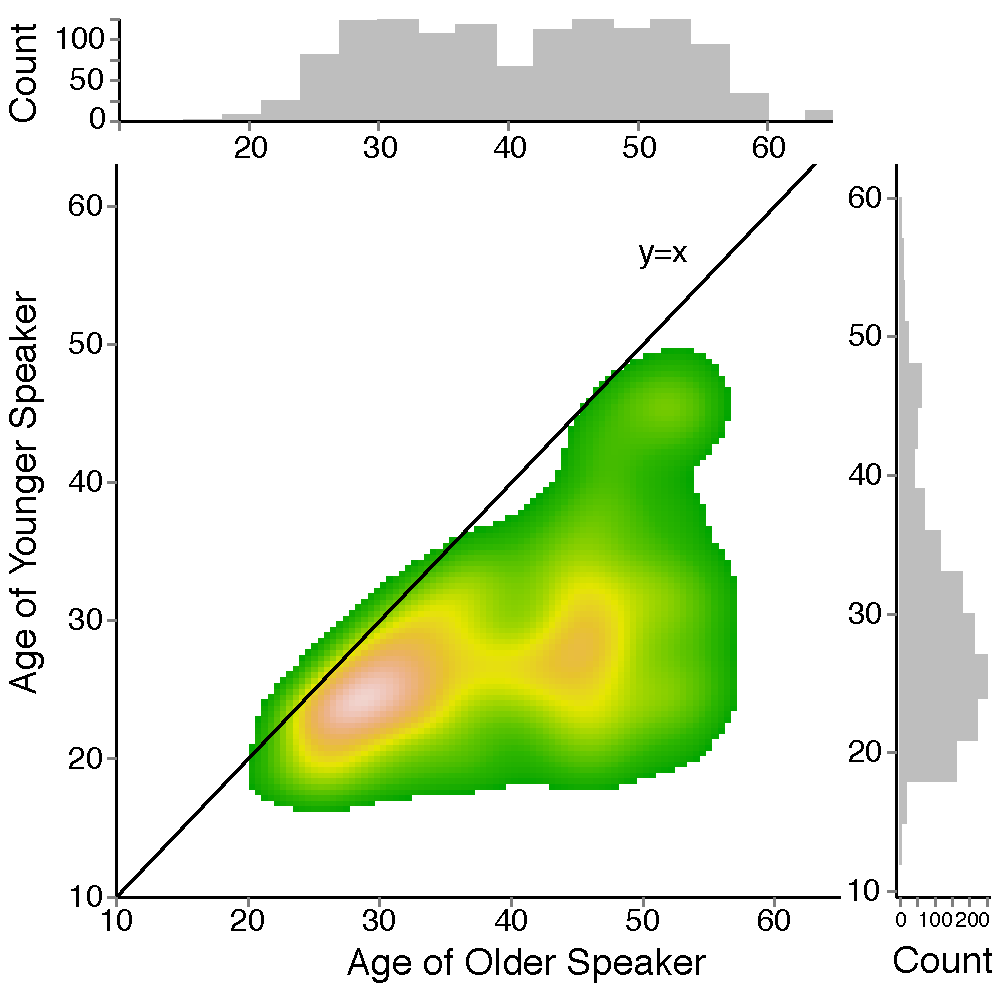
\includegraphics[width=3in]{figures/ageHistogram_edited.pdf}
\caption{ The smoothed joint distribution over ages of younger and older participants in conversations in Switchboard I meeting the sample size requirements for the calculation of lexical overlap. While most conversations occur between a younger speaker between 20 and 30 and an older speaker between 25 and 50, the corpus has appreciable coverage across speaker ages. Measurements are collapsed across the line of symmetry because a conversation between a 32 and a 48 year old speaker is identical to a conversation between a 48 and a 32 year old speaker.}
\label{ageHistogram}
\end{figure}

The Jaccard index, a set theoretic overlap measurement from early work in mathematical ecology \citep{jaccard1912}, provides a conversation-level metric of the proportion of types appearing in the lexical inventories of \textit{both} speakers out of the total number that appeared in \textit{either}. If A and B are sets of lexical types, the Jaccard index is calculated as the cardinality of the set intersection divided  by the cardinality of the set union:

\begin{equation}
\label{eq:Jaccard} 
J(A,B) = \frac{|A\cap B| }{|A\cup B| }
\end{equation}

The Jaccard index is thus a symmetric measurement of overlap ranging from 0 (no shared lexical types) to 1 (only shared lexical types) between speakers: Speaker A cannot be closer to Speaker B than vice versa.

%\footnote{The Dice-S\o renson coefficient statistic, $\frac{2|A\cap B| }{|A| + |B| }$, is a very similar distance metric \citep{dice1945}. The Jaccard index can be derived algebraically from the Dice coefficient   $J = D/(2-D)$.}

\begin{figure*}[t]
\centering
\includegraphics[width=6in]{figures/propRegressions.pdf}
\caption{Left: the Uber index of lexical diversity as a function of speaker age. This measure of lexical diversity reveals that older adults use a more varied vocabulary than younger adults. Right:  Fewer words used by older speakers are used by  their interlocutors. The black line corresponds to the ordinary least squares regression using the single variable depicted. Age values are jittered in the range (+.5,-.5) to minimize overplotting.
} 
\label{propRegressions}
\end{figure*}

For each conversation, we ran 100 independent simulations consisting of drawing 157 tokens with replacement from each speaker and calculating the Jaccard index. The reported Jaccard index was calculated by taking the mean value from these 100 runs.

%Thereafter, the overlap statistic was calculated for each speaker with respect to the other. Unlike the Jaccard index, overlap is an \textit{asymmetric, speaker-level} metric of lexical overlap, defined as the cardinality of the intersection of both speakers' types divided by the cardinality of the target speaker's types (Equations \ref{eq:overlapA} and \ref{eq:overlapB}). This metric can characterize instances where a large promotion of one speaker's types are from a subset of the other. While the Jaccard index is sensitive to whether such an asymmetry exists, it cannot encode its directionality.

%\begin{equation}
%\label{eq:overlapA} 
%overlap(A,B) = \frac{|A\cap B| }{|A| } \\
%\end{equation}
%\begin{equation}
%\label{eq:overlapB} 
%overlap(B,A) = \frac{|A\cap B| }{|B| }
%\end{equation}

%Finally, a new metric of lexical diversity was calculated. In that lexical diversity among samples of a fixed token size can be characterized by the number of types alone ( the numerator in the Uber  index and the left half of the denominator are constants when samples consist of a fixed number of tokens), the number of types is reported as a more intuitive measure than the Uber index (a higher Uber index corresponds to a greater number of types per a fixed number of tokens).


%what are the datasets that are yielded from this procedure?
The above data transformations and measurement procedures produce a dataset with measures of lexical diversity, the number of shared types in a size-controlled sample, and demographic properties for each speaker in each conversation.
Given the dependence of observable behaviors in Switchboard on inherently dyadic communicative processes, we take special care to include demographic properties of the interlocutor along with those of speakers as predictors in our mixed effects models.
%A speaker's lexical diversity can be modeled as a function of the speaker's age, gender, education, dialect, and the topic of conversation; here we additionally examine \textit{interlocutor} age, gender, education, dialect--and the interaction of these with speaker properties---as predictors of a speaker's lexical diversity.
By explicitly treating interlocutor properties as predictors, we can account for contributions of interlocutors to observed speaker behaviors.

%The proportion of shared types in a conversation can thus be treated as a function of  the combined age of the dyad (capturing both young, both old, or mixed dyads in a graded fashion),  the age difference in the dyad,  the pair of speaker gender (both male, both female, or mixed), the combination of dialects, the combined education level, the difference in education, and the topic of conversation.

%\begin{figure}
%\includegraphics[width=3in]{figures/uberRegression.pdf} %this needs a sloper and a model fit
%\caption{Consistent with Horton, Shriberg, and Spieler (2010), the Uber metric of lexical diversity (a variant of the the type-to-token ratio that is robust to differences in sample size) increases with speaker age. 
%} 
%\label{uberRegression}
%\end{figure}

\begin{table*}
\centering
\begin{tabular}{llrrrrl}
\toprule
\multicolumn{2}{l}{}&\multicolumn{1}{c}{Coef $\beta$}&\multicolumn{1}{c}{SE($\beta$)}&\multicolumn{1}{c}{Approx. \textit{df}}&\multicolumn{1}{c}{$t$}&\multicolumn{1}{c}{$Pr(>|t|)$}\tabularnewline
\midrule
& Intercept&$-15.32$&$3.15$&$2765.75$&$-4.86$&\textbf{\textless .0001}\tabularnewline
\hline  \\ [-2ex]
\multirow{13}{*}{Speaker} & Age&$  0.27$&$0.02$&$2741.54$&$12.79$&\textbf{\textless .0001}\tabularnewline
& Gender: Male&$  3.47$&$0.47$&$2764.69$&$ 7.32$&\textbf{\textless .0001}\tabularnewline
& Education: Less than College&$  0.04$&$2.97$&$2743.82$&$ 0.01$&\textgreater .9\tabularnewline
& Education: College&$  3.51$&$2.84$&$2748.28$&$ 1.24$&\textgreater 0.2\tabularnewline
& Education: Some College&$  4.53$&$2.85$&$2749.22$&$ 1.59$&\textgreater 0.1\tabularnewline
& Speaker Education: Unknown&$  7.88$&$3.38$&$2746.50$&$ 2.33$&\textbf{\textless .05}\tabularnewline
& Dialect: New England&$ -2.60$&$1.33$&$2717.47$&$-1.96$&\textgreater 0.1\tabularnewline
& Dialect: North Midland&$ -2.96$&$1.04$&$2737.57$&$-2.83$&\textbf{\textless .01}\tabularnewline
& Dialect: Northern&$ -1.00$&$1.10$&$2732.89$&$-0.90$&\textgreater 0.4\tabularnewline
& Dialect: NYC&$ -3.13$&$1.23$&$2733.32$&$-2.55$&\textbf{\textless .05}\tabularnewline
& Dialect: South Midland&$ -0.59$&$0.96$&$2736.46$&$-0.61$&\textgreater 0.5\tabularnewline
& Dialect: Southern&$ -2.60$&$1.12$&$2732.45$&$-2.32$&\textbf{\textless .05}\tabularnewline
& Dialect: Western&$ -2.70$&$1.07$&$2750.17$&$-2.51$&\textbf{\textless .05}\tabularnewline
\hline  \\ [-2ex]
\multirow{2}{*}{Interlocutor} & Gender: Male&$  1.70$&$0.46$&$2764.48$&$ 3.73$&\textbf{\textless .001}\tabularnewline
& Age&$  0.05$&$0.02$&$2745.18$&$ 2.34$&\textbf{\textless .05}\tabularnewline
\bottomrule
\end{tabular}
\caption{Fixed effects from a linear mixed effects regression model for speaker lexical diversity in which topic was treated as a random effect. Degrees of freedom are calculated according to Satterthwaite's approximation
\citep{satterthwaite1946}.}
\label{lexDivLMER}
\end{table*}

\begin{figure*}[t]
\centering
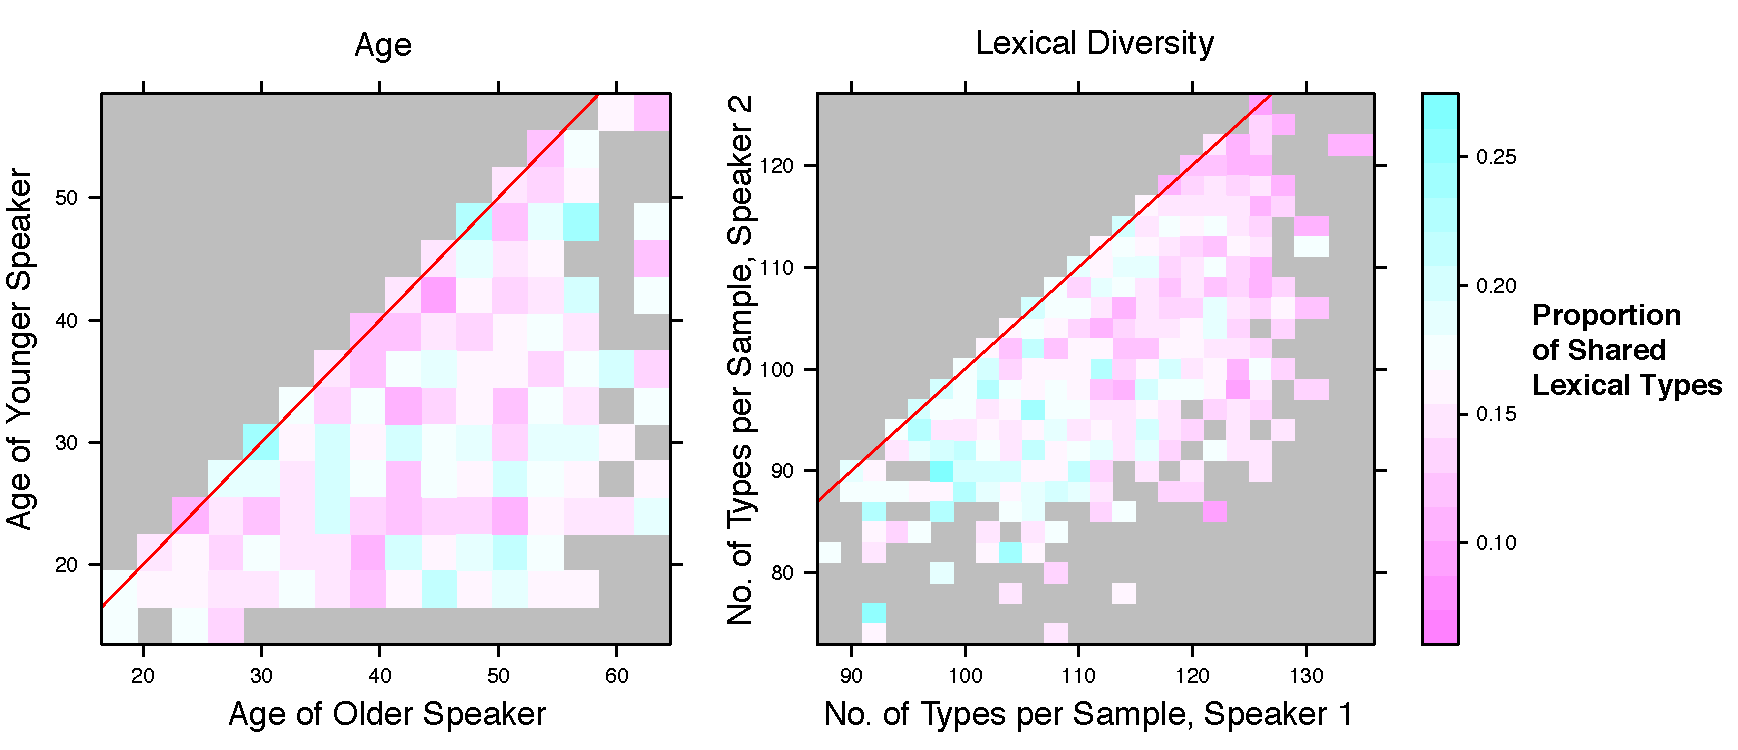
\includegraphics[width=6in]{figures/jaccardsTypesAges.pdf}
\caption{Left: proportion of lexical types shared between speakers in a conversation as a function of the average number of types in samples of a fixed token size. Conversations between speakers with more diverse (within-speaker) lexical inventories exhibit lower proportion of shared lexical types within a conversation. Right:  the same metric of shared lexical types in a conversation as a function of age of speakers. Each pixel represents a mean of observed values in that domain.} 
\label{jaccardTypesAge}
\end{figure*}

\section{Results}
\subsection{Lexical Diversity}
Calculation of the Uber index for all speakers provides for a qualitative replication of the Horton, Shriberg, and Spieler (2010) finding of higher within-subject lexical diversity in the speech of older adults than that of younger adults (Figure \ref{propRegressions}, left). The proportion of lexical types used by a speaker that are also used by his or her interlocutor, a possible but non-obligate correlate of the increase in lexical diversity (see Introduction), decreases with age (Figure \ref{propRegressions}, right). 

% get the t values into this table
\begin{table*}[b]
\centering
\begin{tabular}{lrrrrl}
\toprule
\multicolumn{1}{l}{}&\multicolumn{1}{c}{Coef $\beta$}&\multicolumn{1}{c}{SE($\beta$)}&\multicolumn{1}{c}{Approx. \textit{df}}&\multicolumn{1}{c}{$t$}&\multicolumn{1}{c}{$Pr(>|t|)$}\tabularnewline
\midrule
Intercept&$ 0.0063$&$0.00172$&$ 131.4648$&$ 3.6757$&\textbf{\textless .001}\tabularnewline
Cumulative Age&$-0.0002$&$0.00004$&$1310.0294$&$-5.8097$&\textbf{\textless .0001}\tabularnewline
Female - Male Dyad&$-0.0087$&$0.00166$&$1321.4170$&$-5.2408$&\textbf{\textless .0001}\tabularnewline
Male - Male Dyad&$-0.0120$&$0.00197$&$1331.5834$&$-6.0959$&\textbf{\textless .0001}\tabularnewline
Cumulative Education&$-0.0026$&$0.00084$&$1306.4791$&$-3.1574$&\textbf{\textless .0001}\tabularnewline
\bottomrule
\end{tabular}
\caption{Fixed effects from a linear mixed effects regression model for lexical overlap in conversations in which topic was treated as a random effect.  Degrees of freedom are calculated according to Satterthwaite's approximation \citep{satterthwaite1946}.}
\label{propSharedLMER}
\end{table*}

We constructed a mixed effects linear regression model in which a speaker's lexical diversity, as measured by centered Uber index, was predicted from demographic properties of both the speaker and the interlocutor (age, gender, level of education, and dialect) and the interactions between these properties (Speaker Age $\times$ Interlocutor Age, Speaker Dialect $\times$ Speaker Dialect, etc.) as fixed effects. Conversational topic was treated as a random intercept. This initial model was pruned by comparing the Bayesian Information Criterion (BIC) of the full model against versions of the model with each predictor omitted in turn. Through this procedure, all interaction terms as well as Interlocutor Dialect and Interlocutor Level of Education were removed; the resulting model is displayed in Table \ref{lexDivLMER}.  Age has a small positive $\beta$ coefficient, but is highly reliable. Men tend to exhibit more diverse vocabularies than women in these brief conversations. Lexical diversity increases with level of education, and diversity varies as a function of dialectal variation, though both predictors have high standard error. Interestingly, lexical diversity exhibited by a speaker is dependent on some demographic properties of their interlocutor, possibly because speakers increase or decrease their lexical diversity to match interlocutors in a form of accommodation. Alternatively, interlocutors may directly influence the properties of discourse; for example, an interlocutor may govern the rate at which the conversational dyad moves into new material.
 
\subsection{Proportion of Shared Types}
While age is not a strong predictor of shared lexical types in the absence of additional controls (Figure \ref{jaccardTypesAge}, left), conversations between speakers with high lexical diversity result in a smaller proportion of shared lexical types (Figure \ref{jaccardTypesAge}, right). This decrease in overlap with an increase in lexical diversity suggests speakers do not draw from the same set of types when they exhibit more diverse vocabularies within conversations. Similarly-aged speaker are no more likely to share types (a similarity benefit would manifest as higher values on the diagonal of Figure \ref{jaccardTypesAge}, left).

A linear mixed effects regression model predicting the proportion of shared lexical items (Jaccard's index) per conversation was constructed with topic as a random intercept and cumulative age of the dyad,  the difference in age of the speakers,  male-male, female-female, or mixed speakers, same vs. different dialect speakers, cumulative education, and difference in education, as fixed effects. 
Conversations with one or more speakers with Unknown education levels ($n$=40) were excluded from the analysis, while the remaining levels were treated as a scalar in the range 0-3.
Stepwise model pruning on the basis of BIC supported the exclusion of difference terms and dialectal properties of speakers from the final model (Table \ref{propSharedLMER}).
Older dyads exhibited marginally higher proportions of shared types than younger ones. Male and female dyads exhibit fewer shared types than female-female dyads; male-male dyads exhibit even lower type overlap. Higher levels of education were predictive of a lower Jaccard index. 


%\begin{figure*}
%\centering
%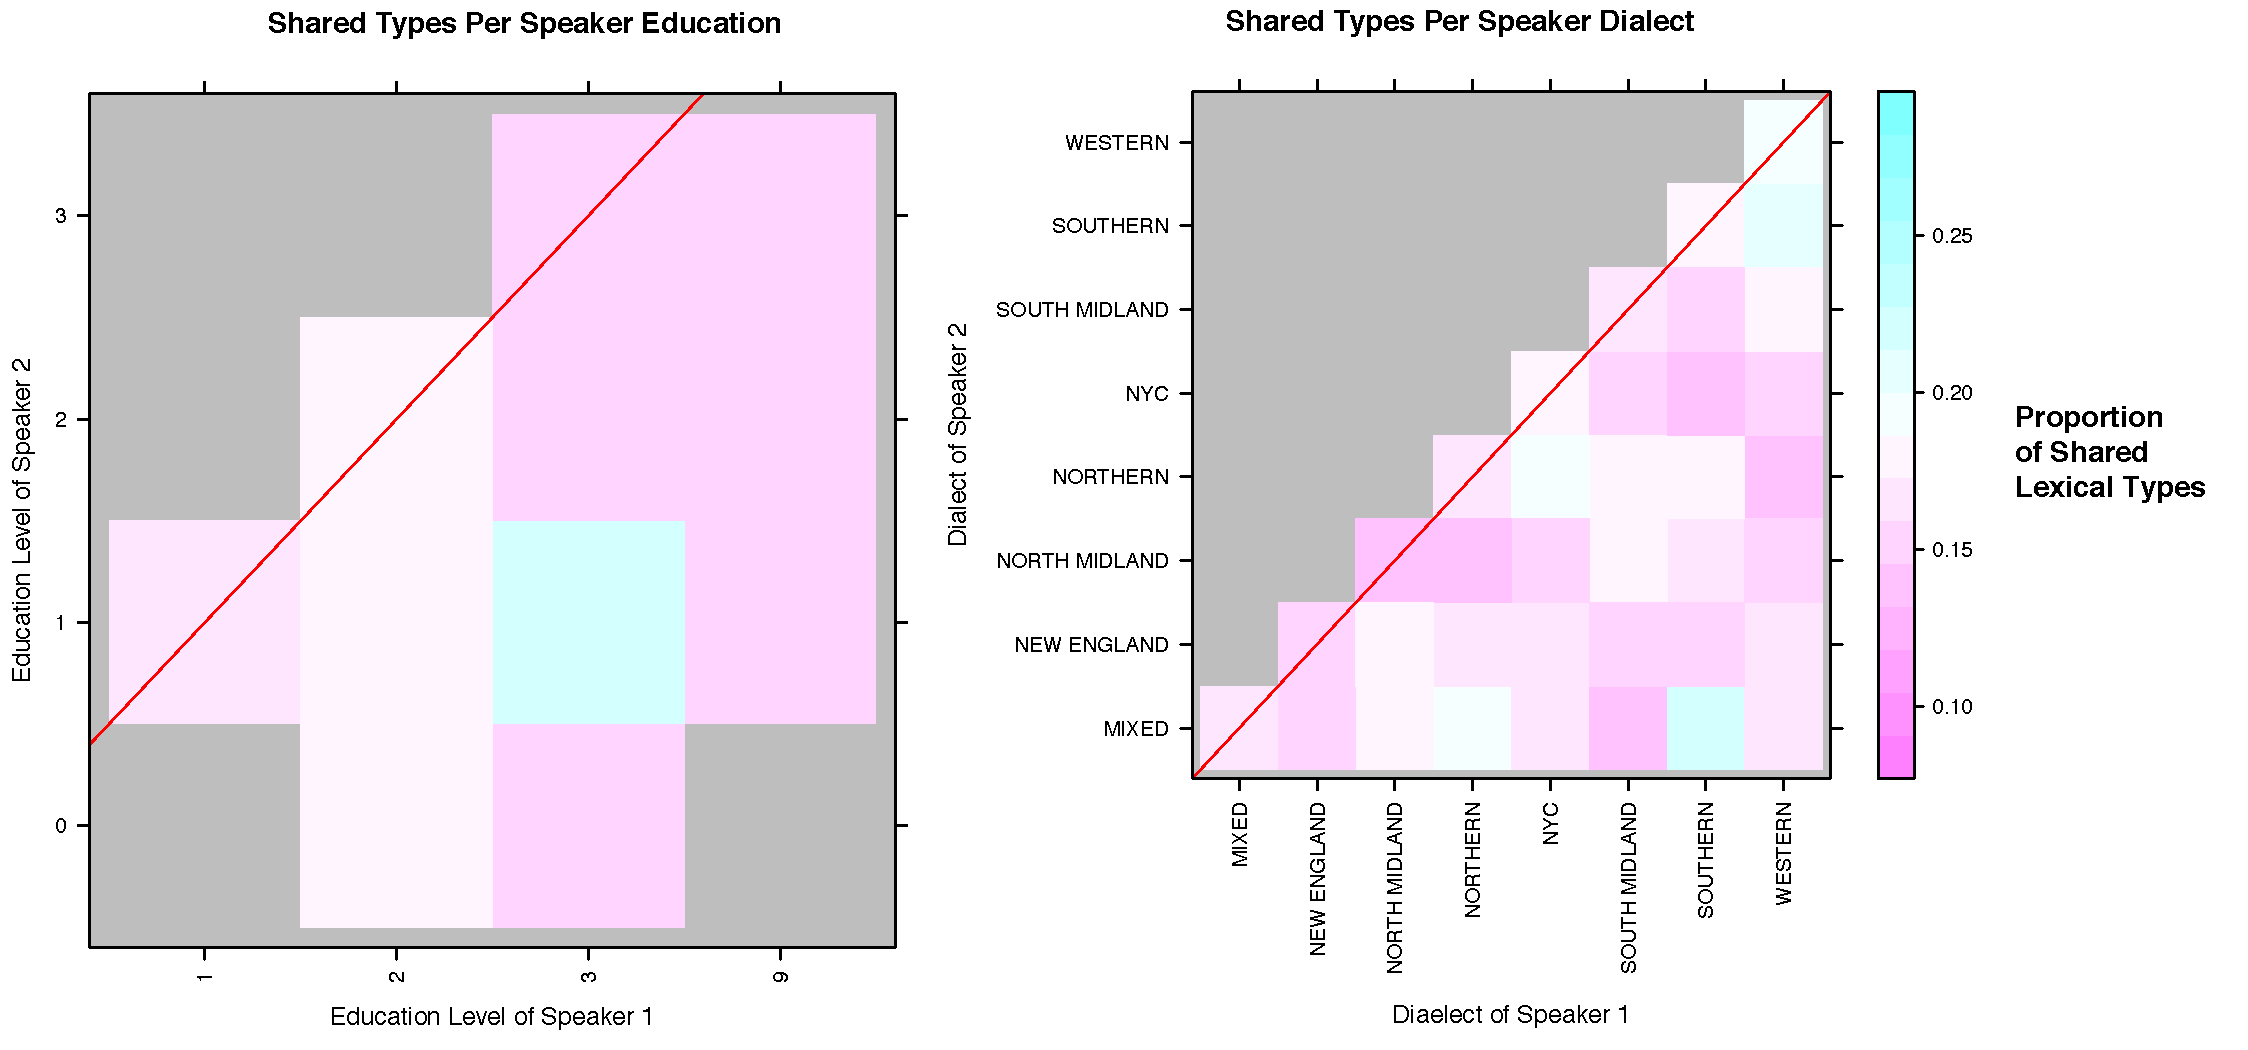
\includegraphics[width=6in]{figures/jaccardsEducationDialect.pdf}
%\caption{Left: proportion of lexical types shared between speakers as a function of education level of the interlocutors. Right:  proportion of lexical types shared between speakers as a function of dialect region. In both cases, the absence of higher values on the diagonal suggests that speakers with similar backgrounds are no more likely to use the same lexical items conversations than speakers with varying backgrounds.} 
%\label{jaccardEducationDialect}
%\end{figure*}

\section{Limitations And Future Work}
The lexical inventory of a speaker in a brief telephone conversation is necessarily modulated by the particular communicative needs of that conversation. While the current work suggests that properties of speaker identity have a detectable effect on lexical diversity \textit{despite} the brevity of conversations and discourse-specific effects, corpora with longer interactions between speakers and more conversations per speaker could allow for better decoupling of speaker-specific effects from discourse-specific effects.
%random slope for subject?  

The current work excluded function words from the analysis because of extremely high levels of overlap between subjects. ``A,'' ``I,'' and, ``the,'' for example, were used by virtually every speaker in the sample. However, the blanket exclusion of function word, including relatively low frequency function words like ``although'' and ``moreover,''  removes a potentially interesting source of lexical variability between speakers and age groups. Given previous work on gendered differences in the use of function words \citep{newmanEtAl2008}, we might expect even greater gender-based effects in lexical overlap than those observed here.

% Pronouns, posited to be an index of common ground \citep{clark:1996}, might also be a fruitful area of investigation, though how to correctly calculate overlap is not altogether straightforward in situations of deixis (i.e. one speaker's ``my'' is in some sense equivalent to an interlocutor's ``your'').

Another shortcoming of the current method is that it treats each conversation as a single temporal point, and neglects variability within the timecourse of the conversation.
No strong conclusions may be drawn regarding processes of lexical accommodation, wherein speakers display increasing or decreasing levels of similarity in lexical choice over the course of the conversation.
Comparison of size-matched temporal subsets would further reduce the number of analyzable tokens; as such new metrics for calculating between speaker lexical overlap may be required to elucidate within-conversation dynamics.

\section{Conclusion}
The current work leaves us with a consistent picture of lexical diversity and overlap in conversational speech.
A speaker's lexical diversity is conditioned on the properties of his or her interlocutor, but age and higher levels of education predict increased lexical diversity for individual speakers. 
Within-speaker type inventories that are more diverse result in fewer shared lexical items in conversations. Consistent with predictions derived from \citet{ramscarEtAl2014} regarding lifelong learning, older speakers use more word types than younger speakers, and their particular selection of words is more likely to diverge with other older speakers. That such patterns are identifiable even in brief samples of conversational speech suggests that lifelong changes in language production may be implicated even in short episodes of everyday language use.

%\section{Code}
%R language source code for data processing, figure generation, and regressions can be downloaded from \url{https://github.com/smeylan/swbd}.

%\section{Acknowledgments}
%This material is based upon work supported by the National Science Foundation Graduate Research Fellowship under Grant No. DGE-1106400.

\bibliographystyle{apacite}

\setlength{\bibleftmargin}{.125in}
\setlength{\bibindent}{-\bibleftmargin}

\def\thebibliography#1{\section*{References}
 \small
  \list
  {[\arabic{enumi}]}{\leftmargin \parindent
    \itemindent -\parindent
    \itemsep 0ex plus 1pt
    \parsep 0.1ex plus 1pt minus 1pt
    \usecounter{enumi}}
    \def\newblock{\hskip .11em plus .33em minus .07em}
    \sloppy\clubpenalty4000\widowpenalty4000
    \sfcode`\.=1000\relax}


\bibliography{lexDivergence_bibliography}



\end{document}
